\documentclass{beamer}

%%% ISSUE BBB solved %%%
%\usepackage{lmodern}
%%%%%%%%%%%%%%%%%%%%%%%%

\usepackage[utf8]{inputenc}
\usepackage[T1]{fontenc}
\usepackage{multicol}
\usepackage{amsthm}
\usepackage{amsmath}
\usepackage{amssymb}
\usepackage{mathtools}
\usepackage{dsfont}
\usepackage{bm}
\usepackage{bbm}
\usepackage{xparse}
\usepackage{physics}
\usepackage{empheq}
\usepackage{url}
\usepackage{hyperref}
%\usepackage[affil-it]{authblk}
%\usepackage{enumitem}
\usepackage{rotating}
\usepackage{graphicx}
\usepackage[linesnumbered,ruled,vlined]{algorithm2e}

\usepackage{tikz}
\usetikzlibrary{calc}
\usetikzlibrary{shapes,arrows,snakes}

\tikzstyle{block} = [draw, fill=white, rectangle, 
  minimum height=2em, minimum width=3em]
\tikzstyle{bigblock} = [draw, fill=white, rectangle, 
  minimum height=3em, minimum width=4em]
\tikzstyle{Bigblock} = [draw, fill=white, rectangle, 
    minimum height=5em, minimum width=8.5em]
\tikzstyle{input} = [coordinate]
\tikzstyle{output} = [coordinate]
\tikzstyle{pinstyle} = [pin edge={to-,thin,black}]

\usepackage{pgfplots}
\pgfplotsset{compat = newest}

\theoremstyle{definition}
\newtheorem{theo}{Theorem}[section]
\newtheorem{lem}[theo]{Lemma}
\newtheorem{cor}[theo]{Corollary}
\newtheorem{prop}[theo]{Proposition}
\newtheorem{defi}[theo]{Definition}
\newtheorem{conj}[theo]{Conjecture}

\newtheorem{theo*}{Theorem}

\theoremstyle{remark}
\newtheorem*{rk}{Remark}

\DeclareMathOperator{\Poi}{\text{Poi}}
\DeclareMathOperator{\Ber}{\text{Ber}}
\DeclareMathOperator{\Bin}{\text{Bin}}
\DeclareMathOperator{\maxi}{\text{maximize}}
\DeclareMathOperator{\mini}{\text{minimize}}
\DeclareMathOperator{\st}{\text{subject to}}
\DeclarePairedDelimiter\ceil{\lceil}{\rceil}
\DeclarePairedDelimiter\floor{\lfloor}{\rfloor}
\DeclarePairedDelimiterX\set[1]\lbrace\rbrace{\def\given{\;\delimsize\vert\;}#1}

\colorlet{darkgreen}{green!40!black}
\colorlet{lightred}{red!60!white}

\usepackage{appendixnumberbeamer}
\beamertemplatenavigationsymbolsempty

%%%%%%%%%
\usetheme{Dresden}
\usecolortheme{lily}
\newcommand*\oldmacro{}%
\let\oldmacro\insertshorttitle%
\renewcommand*\insertshorttitle{%
  \oldmacro\hfill%
  \insertframenumber\,/\,\inserttotalframenumber}
%%%%%%%%%



\title{Approximation Algorithms for Channel Coding and Non-Signaling Correlations}
\subtitle{\textit{Algorithmes d'approximation pour le problème du codage de canal et corrélations non-signalantes}}
\author{Paul Fermé}
\institute{ENS de Lyon}
\date{29 novembre 2023}

%\AtBeginSection[]
%{
%  \begin{frame}<beamer>
%    \frametitle{Contents}
%    \tableofcontents[currentsection]
%  \end{frame}
%}

%%%%%%%%%%%%%%%%%%%%%%%%%%%%%%%%%%%%%%%%%%
\begin{document}
%%%%%%%%%%%%%%%%%%%%%%%%%%%%%%%%%%%%%%%%%%

\begin{frame}
  \titlepage
\end{frame}


\section{Introduction}
\subsection{Le problème du codage de canal}
\begin{frame}{Qu'est ce qu'un canal de communication ?}
  \pause
  \begin{center}
    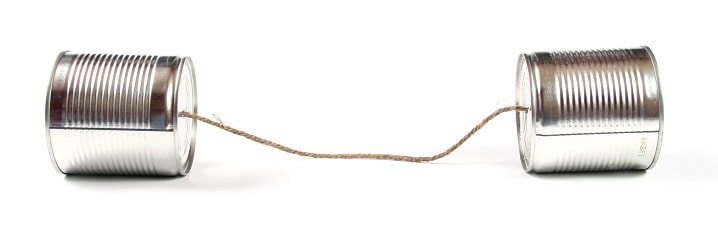
\includegraphics[scale=0.42]{tin-can-telephone.jpg}
    
      \pause
      Vent ? Pluie ? Obstacles ?
  \end{center}
\end{frame}

\begin{frame}{Communiquer avec du bruit ?}
  \begin{center}
  \begin{tikzpicture}
    %%% Tin can telephone %%%
    \node at (4.7,0) (tin) {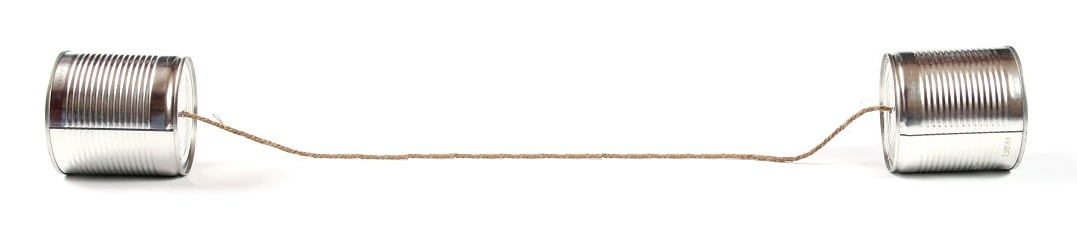
\includegraphics[scale=0.22]{long-tin-can-telephone.jpg}};

    %%% Left callouts %%%
    \only<1-2>{\node[ellipse callout, draw, callout relative pointer={(-0.3,-0.3)}] at (-0.1,0.1) (Alice) {\Large Allô!};}
    \only<3>{\node[ellipse callout, draw, callout relative pointer={(-0.3,-0.3)}] at (-0.1,2.1) (Alice) {\Large \alert{A}llô!};
      \node[ellipse callout, draw, callout absolute pointer={(-0.1,1.5)}] at (-0.1,0.1) (Alice) {Alfa};}
    \only<4>{\node[ellipse callout, draw, callout relative pointer={(-0.3,-0.3)}] at (-0.1,2.1) (Alice) {\Large A\alert{l}lô!};
      \node[ellipse callout, draw, callout absolute pointer={(-0.1,1.5)}] at (-0.1,0.1) (Alice) {Lima};}
    \only<5>{\node[ellipse callout, draw, callout relative pointer={(-0.3,-0.3)}] at (-0.1,2.1) (Alice) {\Large Al\alert{l}ô!};
      \node[ellipse callout, draw, callout absolute pointer={(-0.1,1.5)}] at (-0.1,0.1) (Alice) {Lima};}
    \only<6>{\node[ellipse callout, draw, callout relative pointer={(-0.3,-0.3)}] at (-0.1,2.1) (Alice) {\Large All\alert{ô}!};
      \node[ellipse callout, draw, callout absolute pointer={(-0.1,1.5)}] at (-0.1,0.1) (Alice) {\small Oscar};}
    %%% Cloud %%%
    \only<1>{\node at (4.6,1.5) (wcloud) {
\includegraphics[scale=0.3]{rcloud_white.png}};}
    \only<2-6>{\node at (4.6,1.5) (cloud) {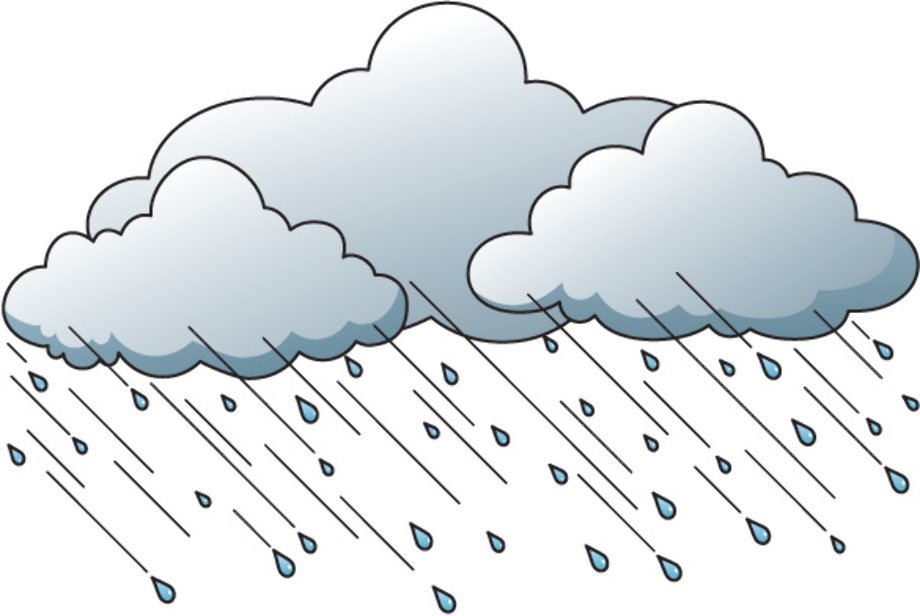
\includegraphics[scale=0.3]{rcloud.png}};}

    %%% Right callouts %%%
    \only<1>{\node[ellipse callout, draw, callout relative pointer={(-0.2,0)}] at (9.7,0.1) (Bob) {\Large Allô!};}
    \only<2>{\node[dashed, ellipse callout, draw, callout relative pointer={(-0.2,0)}] at (9.7,0.1) (Bob) {\tiny Ah, l'eau!};}
    \only<3>{\node[dashed, ellipse callout, draw, callout relative pointer={(-0.2,0)}] at (9.4,0.1) (Bob) {\tiny Alma};
      \node[ellipse callout, draw, callout absolute pointer={(9.4,0.5)}] at (9.4,2.1) (Alice) {\Large \alert{A}};}
    \only<4>{\node[dashed, ellipse callout, draw, callout relative pointer={(-0.2,0)}] at (9.4,0.1) (Bob) {\tiny Lena};
      \node[ellipse callout, draw, callout absolute pointer={(9.4,0.5)}] at (9.4,2.1) (Alice) {\Large A\alert{L}};}
    \only<5>{\node[dashed, ellipse callout, draw, callout relative pointer={(-0.2,0)}] at (9.4,0.1) (Bob) {\tiny Rima};
      \node[ellipse callout, draw, callout absolute pointer={(9.4,0.5)}] at (9.4,2.1) (Alice) {\Large AL\alert{L}};}
    \only<6>{\node[dashed, ellipse callout, draw, callout relative pointer={(-0.2,0)}] at (9.5,0.1) (Bob) {\tiny Lascar};
      \node[ellipse callout, draw, callout absolute pointer={(9.5,0.5)}] at (9.5,2.1) (Alice) {\Large ALL\alert{O}};}
  \end{tikzpicture}
  \end{center}
\end{frame}


\begin{frame}{Modélisation mathématique}
  \begin{center}
    \begin{tikzpicture}[auto, node distance=2cm,>=latex']
      \node [bigblock] (W) {\only<1-2>{$W$}\only<3>{$6/10$}\only<4>{$3/10$}\only<5>{$1/10$}};
      \node [right of=W] (y) {\only<1-2>{$y$}\only<3>{\emph{alfa}}\only<4>{\emph{alma}}\only<5>{\emph{alvo}}};
      \node [left of=W] (x) {\only<1-2>{$x$}\only<3-5>{\emph{alfa}}};
      \draw [->] (x) -- (W);
      \draw [->] (W) -- (y);
    \end{tikzpicture}

    \pause
    \bigskip
    Probabilité \only<2>{$W(y|x)$}\only<3>{$6/10$}\only<4>{$3/10$}\only<5>{$1/10$} d'avoir la sortie \only<2>{$y$}\only<3>{\emph{alfa}}\only<4>{\emph{alma}}\only<5>{\emph{alvo}} pour l'entrée \only<2>{$x$}\only<3-5>{\emph{alfa}}
  \end{center} 
\end{frame}

\begin{frame}{Le problème du codage de canal}
  \begin{center}
    \begin{tikzpicture}[auto, node distance=2.5cm,>=latex']
      \node [block] (e) {$e$};
      \node [bigblock, right of=e] (W) {\only<1,5>{$W$}\only<2>{$6/10$}\only<3>{$3/10$}\only<4>{$1/10$}};
      \node [block, right of=W] (d) {$d$};
      \draw [->] (e) -- node[name=x] {\only<1,5>{$x$}\only<2-4>{\emph{alfa}}} (W);
      \draw [->] (W) -- node[name=y] {\only<1,5>{$y$}\only<2>{\emph{alfa}}\only<3>{\emph{alma}}\only<4>{\emph{alvo}}} (d);
      \node [left of=e, node distance=1.5cm] (i) {\only<1>{$i$}\only<2-4>{\alert{a}}\only<5>{\alert{b,\ldots,z}}};
      \node [right of=d,  node distance=1.5cm] (j) {\only<1>{$j$}\only<2-3>{\alert{a}}\only<4>{\alert{b}}\only<5>{\alert{b,\ldots,z}}};
      \draw [draw,->] (i) -- (e);
      \draw [draw,->] (d) -- (j);
    \end{tikzpicture}

    \bigskip

    Trouver $e$ et $d$ qui maximise la probabilité d'avoir $j=i$\only<5>{\ldots\\
      \bigskip
      \ldots sur tout l'alphabet (noté $[k]$; ici $k=26$) !
      \[ \text{\underline{Formellement:} } \underset{e,d}{\max} \ \frac{1}{k} \sum_{i,x,y} e(x|i)W(y|x)d(i|y) \]
    }
  \end{center}
\end{frame}

\begin{frame}{Résolution \cite{BF18}}
  \begin{itemize}
  \item \underline{Objectif:} méthode systématique (algorithme) pour trouver les meilleurs $e,d$ pour un $W$.
    \pause
  \item \underline{Problème:} impossible (\textrm{NP}-difficulté) de créer un algorithme efficace (temps polynomial) qui trouve ces $e,d$.
    \bigskip
    \pause
  \item \underline{Solution:} plutôt que les meilleurs $e,d$, on se contente d'un choix de $e,d$ avec une valeur \emph{proche} des meilleurs.
    
    \pause
    \bigskip

  \item \cite{BF18}: approximation qui garantit au moins $\simeq 63\%$ (coefficient $1-e^{-1}$) aussi bien que les meilleurs.
  \item Impossible (\textrm{NP}-difficile) de faire mieux que $1-e^{-1}$.
  \end{itemize}
\end{frame}

\begin{frame}{Décodage de liste}
  \begin{center}
    \begin{tikzpicture}[auto, node distance=2.5cm,>=latex']
      \node [block] (e) {$e$};
      \node [bigblock, right of=e] (W) {\only<1,3-6>{$W$}\only<2>{$1/10$}};
      \node [block, right of=W] (d) {$d$};
      \draw [->] (e) -- node[name=x] {\only<1,3-6>{$x$}\only<2>{\emph{alfa}}} (W);
      \draw [->] (W) -- node[name=y] {\only<1,3-6>{$y$}\only<2>{\emph{alvo}}} (d);
      \node [left of=e, node distance=1.5cm] (i) {\only<1,3-6>{$i$}\only<2>{\alert{a}}};
      \node [right of=d,  node distance=2cm] (j) {\only<1>{$[j_1,j_2]$}\only<2>{\alert{[a,b]}}\only<3-6>{$[j_1,j_2,\ldots,j_{\ell}]$}};
      \draw [draw,->] (i) -- (e);
      \draw [draw,->] (d) -- (j);
    \end{tikzpicture}

    \bigskip
    Trouver $e,d$ qui maximise la probabilité que \only<1-2>{$j_1$ ou $j_2$}\only<3-6>{$j_1,j_2,\ldots$ ou $j_{\ell}$} égal à $i$.
  \end{center}
  
  \pause\pause\pause
  
  \begin{itemize}
  \item \cite{BFGG20}: Algorithme d'approximation avec un facteur $1-\frac{\ell^{\ell}e^{-\ell}}{\ell!}$ (pour $\ell=2$, correspond à $\simeq 73\%$).
    \pause
  \item On va montrer que c'est \textrm{NP}-difficile de faire mieux.
    \pause
  \item On va étudier une généralisation, où la taille $\ell$ de la liste n'est pas fixée, mais vient avec une pénalité $\frac{\varphi(\ell)}{\ell}$.
  \end{itemize}
\end{frame}

\subsection{Les corrélations non-signalantes}
\begin{frame}{La physique quantique\only<3>{\ldots et ses idées reçues}}
  \begin{center}
    \pause
  \begin{tikzpicture}
    %%% Tin can telephone %%%
    \node at (0,0) (cat_ud) {
\includegraphics[scale=0.1]{cat_upsidedown.png}};
    \node at (5,0) (cat_ud) {
\includegraphics[scale=0.1]{cat_downupside.png}};
    \node[scale=0.5, align=center, ellipse callout, draw, fill=white, callout relative pointer={(0.7,-0.3)}] at (-0.1,0) (upside) {J'ai la tête\\ en bas.};
    \node[scale=0.5, align=center, ellipse callout, draw, fill=white, callout relative pointer={(-0.7,0.3)}] at (5.1,0) (upside) {J'ai la tête\\ en haut.};

    \only<2>{\node at (2.5,-3.5) (cat_q) {
\includegraphics[scale=0.12]{cat_question_white.png}};}
    \only<3>{\node at (2.5,-3.5) (cat_q) {
\includegraphics[scale=0.12]{cat_question.png}};
      \node[scale=0.5, align=center, ellipse callout, draw, fill=white, callout relative pointer={(0.6,-0.6)}] at (2.7,-2.4) (Notallowed) {J'ai rien\\ à faire là!};
    }
  \end{tikzpicture}
  \end{center}
\end{frame}

\begin{frame}{De quoi parle la physique quantique ?}
  \begin{itemize}
  \item Comprendre physique à l'\emph{échelle} des atomes -- \emph{un million de fois plus petit qu'un grain de sable !} (0,1nm)
    \begin{center}
      \begin{tikzpicture}
        \node at (0,0) (atom1) {
\includegraphics[scale=0.04]{atom.jpg}};
        \node at (3,0) (atom2) {
\includegraphics[scale=0.04]{atom.jpg}};
        \only<3-4>{\draw[snake=coil, segment aspect=0, red] (0,0) -- (3,0);}
      \end{tikzpicture}
    \end{center}
    \pause
  \item Phénomène spécifique à cette échelle...\pause \alert{l'intrication quantique :}
    \pause
    \\ \ 
    \begin{center}
      \alert{Deux particules \emph{corrélées} à très grande distance\\
      \emph{Inexplicable} par physique non quantique !}
    \end{center}
  \end{itemize}
\end{frame}

\begin{frame}{Le paradoxe Einstein-Podolski-Rosen}

  \begin{itemize}
  \item \underline{Années 1920 :} naissance de la physique quantique
    \pause
    \bigskip
  \item \underline{Paradoxe EPR~\cite{EPR35} :} deux particules intriquées à distance
    \begin{center}
      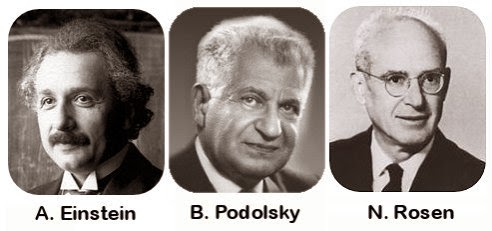
\includegraphics[scale=0.3]{EPR.jpg}
    \end{center}
    \pause
    \begin{enumerate}
    \item Soit contradiction avec le \emph{principe de localité}
    \item Soit mécanique quantique \emph{incomplète} (variables cachées)
    \end{enumerate}
    \pause
  \item De manière inattendue, c'est \alert{le premier} qui décrit la réalité !
  \item Communication plus rapide que la lumière ? \pause{\alert{\emph{Non, corrélations !}}}
  \end{itemize}
\end{frame}

\begin{frame}{Inégalités de Bell et expérience d'Aspect}
  \begin{itemize}
  \item \underline{Inégalités de Bell~\cite{Bell64} :} expérience distinguant corrélations :\begin{enumerate}
    \item causées par de l'intrication quantique
    \item provenant de variables cachées
  \end{enumerate}
  \end{itemize}
  \pause
  \begin{columns}
    \begin{column}{2cm}
      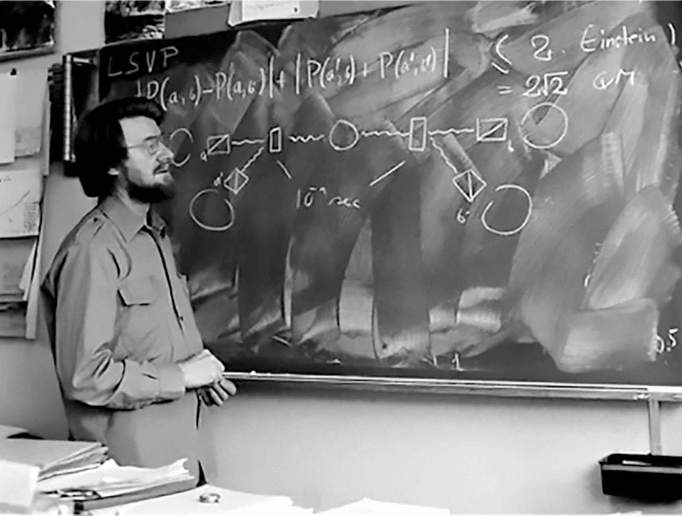
\includegraphics[scale=0.15]{BellAspect.png}
    \end{column}
    \begin{column}{6cm}
      \begin{itemize}
      \item \underline{Expérience d'Aspect~\cite{ADG82} :} réalisation pratique de cette expérience.
      \end{itemize}
    \end{column}
    \end{columns}
    \pause
    \bigskip
    \begin{itemize}
  \item \underline{Expérience QUESS~\cite{Yin17} :} intrication entre particules à 1200 km de distance
  \end{itemize}
\end{frame}

\begin{frame}{Le jeu CHSH}
  \begin{center}
    \only<2->{On tire $x,y$ au hasard dans $\{0,1\}$, on les donne à Alice et Bob.\\}
    \bigskip
   \begin{tikzpicture}[auto, node distance=1.8cm,>=latex']
      \node [block] (A) {
\includegraphics[scale=0.08]{Alice.png}};
      \only<2->{\node [above of=A] (x) {$x$};
      \draw [->] (x) -- (A);}
      \only<3->{\node [below of=A] (a) {$\alert{a}$};
      \draw [->] (A) -- (a);}

      \node [right of=A] (I) {};
      \only<4->{\node [color=blue,above of=I,outer sep=0pt,circle,fill,inner sep=1pt] (Iabove) {};
      \node [color=blue,below of=I,outer sep=0pt,circle,fill,inner sep=1pt] (Ibelow) {};
      \draw [color=blue,dotted, thick] (Iabove) -- (Ibelow);}
      
      \node [block, right of=I] (B) {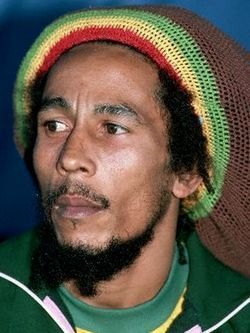
\includegraphics[scale=0.16]{Bob.jpg}};
      \only<2->{\node [above of=B] (y) {$y$};
      \draw [->] (y) -- (B);}
      \only<3->{\node [below of=B] (b) {$\alert{b}$};
      \draw [->] (B) -- (b);}

      \only<7>{\node [starburst, fill=white, draw=lightred, line width=1pt, text=red] at (I) {\Large $3/4$};}
   \end{tikzpicture}
   \bigskip
   \\
   \only<3-4>{Alice et Bob choisissent $\alert{a}$ et $\alert{b}$ dans $\{0,1\}$\only<4->{, \textcolor{blue}{sans communiquer !}}\\\bigskip}
   \only<5->{\underline{Objectif :} Si $x=y=1$, alors $\alert{a}\not=\alert{b}$ ; sinon $\alert{a}=\alert{b}$.\\\bigskip}
   \only<6->{\large\emph{Quelle est la probabilité de succès de la meilleure stratégie ?}}
  \end{center}
\end{frame}

\begin{frame}{Variables cachées, intrication quantique et non-signalante}
  \begin{center}
    Et si Alice et Bob partagent\ldots\only<2-4>{des \textcolor{blue}{\emph{variables cachées}} ?}\only<5-7>{de \textcolor{blue}{\emph{l'intrication quantique}} ?}\only<8->{des \textcolor{blue}{\emph{corrélations non-signalantes}} ?}\\\bigskip
    \begin{tikzpicture}[auto, node distance=1.8cm,>=latex']
      \node [block] (A) {
\includegraphics[scale=0.08]{Alice.png}};
      \node [above of=A] (x) {$x$};
      \draw [->] (x) -- (A);
      \node [below of=A] (a) {$\alert{a}$};
      \draw [->] (A) -- (a);

      \node [right of=A] (I) {};
      \node [color=blue,above of=I,outer sep=0pt,circle,fill,inner sep=1pt] (Iabove) {};
      \node [color=blue,below of=I,outer sep=0pt,circle,fill,inner sep=1pt] (Ibelow) {};
      \draw [color=blue,dotted, thick] (Iabove) -- (Ibelow);
      
      \node [block, right of=I] (B) {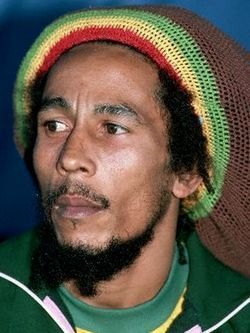
\includegraphics[scale=0.16]{Bob.jpg}};
      \node [above of=B] (y) {$y$};
      \draw [->] (y) -- (B);
      \node [below of=B] (b) {$\alert{b}$};
      \draw [->] (B) -- (b);

      \only<2->{
        \draw [snake=coil,segment aspect=0, draw=blue] (A) -- (B);
        \node [circle, fill=white, draw=blue, text=blue] at (I) (Corr) {\only<2-4>{$\lambda$}\only<5-7>{$\varphi$}\only<8->{\textrm{NS}}};}
      \only<4>{\node [starburst, fill=white, draw=lightred, line width=1pt, text=red] at (I) {\Large $3/4$};}
      \only<7>{\node [starburst, fill=white, draw=lightred, line width=1pt, text=red] at (I) {\Large $85\%$};}
      \only<11>{\node [starburst, fill=white, draw=lightred, line width=1pt, align=left, text=red] at (I) {Encore\\ mieux !};}
    \end{tikzpicture}\\\bigskip
    
    \only<3-4>{\emph{Avant l'expérience}, s'accordent sur un \textcolor{blue}{$\lambda$} aléatoire.\\
      Alice et Bob peuvent l'utiliser \emph{tous les deux} pour choisir $\alert{a}$ et $\alert{b}$.}
    \only<6-7>{Toujours \textcolor{blue}{pas de communication} ! Stratégie $P(\alert{ab}\textcolor{blue}{\textbf{|}}xy)$ vérifie que :\\
      $\alert{a}$ \textcolor{blue}{ne dépend pas de} $y$ et $\alert{b}$ \textcolor{blue}{ne dépend pas de} $x$.}
    \only<9->{\emph{Toutes les stratégies $P(\alert{ab}\textcolor{blue}{\textbf{|}}xy)$ \textcolor{blue}{sans communication}}, càd telles que :\\}
    \only<9>{$\alert{a}$ \textcolor{blue}{ne dépend pas de} $y$ et $\alert{b}$ \textcolor{blue}{ne dépend pas de} $x$.}
    \only<10->{$P(\alert{a}|xy)=P(\alert{a}|xy')$ et $P(\alert{b}|xy)=P(\alert{b}|x'y)$.}
  \end{center}
\end{frame}

\begin{frame}{Assistance non-signalante pour le codage de canal}
  \begin{center}
    \begin{tikzpicture}[auto, node distance=1.6cm,>=latex']
      \only<1>{\node [bigblock] (W) {$W$};
        \node [left of=W] (x) {$x$};
        \node [block,left of=x] (e) {$e$};
        \node [left of=e] (i) {$i$};
        \node [right of=W] (y) {$y$};
        \node [block,right of=y] (d) {$d$};
        \node [right of=d] (j) {$j$};
        \draw [->] (i) -- (e);
        \draw [->] (e) -- (x);
        \draw [->] (x) -- (W);
        \draw [->] (W) -- (y);
        \draw [->] (y) -- (d);
        \draw [->] (d) -- (j);}

      \only<2->{\node [block] (A) {$e$};
      \node [above of=A] (x) {$i$};
      \draw [->] (x) -- (A);
      \node [below of=A] (a) {\only<2>{$x$}\only<3->{$\alert{x}$}};
      \draw [->] (A) -- (a);

      \node [right of=A] (I) {};
      
      \node [block, right of=I] (B) {$d$};
      \node [above of=B] (y) {$y$};
      \draw [->] (y) -- (B);
      \node [below of=B] (b) {\only<2>{$j$}\only<3->{$\alert{j}$}};
      \draw [->] (B) -- (b);
      
      \node [dashed,right of=B] (Bright) {};
      \node [dashed,bigblock,right of=Bright] (W) {$W$};
      \draw [dashed,->] (a) to[out=-20,in=-90] (W);
      \draw [dashed,->] (W) to[out=90,in=20] (y);}

      
      \only<3->{\node [color=blue,above of=I,outer sep=0pt,circle,fill,inner sep=1pt] (Iabove) {};
      \node [color=blue,below of=I,outer sep=0pt,circle,fill,inner sep=1pt] (Ibelow) {};
      \draw [color=blue,dotted, thick] (Iabove) -- (Ibelow);
      \draw [snake=coil,segment aspect=0, draw=blue] (A) -- (B);
      \node [circle, fill=white, draw=blue, text=blue] at (I) (Corr) {\textrm{NS}};}
    \end{tikzpicture}\\
    \only<2>{On peut considérer la stratégie encodage-décodage indépendamment de $W$ !}
    \only<3>{La stratégie encodage-décodage est décrite par $P(\alert{xj}\textcolor{blue}{\textbf{|}}iy)$ :\\
      Calcul de $e(\alert{x}|i)$ \textcolor{blue}{sans} $y$ ; corrélation \emph{\alert{globale}} inexplicable \emph{localement}.}
    \only<4>{\underline{\cite{BF18} :}  meilleure communication (jusqu'à $58\%$ ($\frac{e^{-1}}{1-e^{-1}}$)), mais pas de changement de \emph{capacité} du canal.}
  \end{center}
\end{frame}

\begin{frame}{Canaux en réseaux}
    \begin{center}
      \begin{tikzpicture}[auto, node distance=2cm,>=latex']
        \only<1>{\node [bigblock] (W) {$W$};
          \node [right of=W] (y) {$y$};
          \node [left of=W] (x) {$x$};
          \draw [->] (x) -- (W);
          \draw [->] (W) -- (y);
          \node [below of=W] (txt) {Canal un-à-un};}

        \only<2->{\node [bigblock] (Wa) {$W$};
          \node [above right of=Wa] (y1) {$y_1$};
          \node [below right of=Wa] (y2) {$y_2$};
          \node [left of=Wa] (x) {$x$};
          \draw [->] (x) -- (Wa);
          \draw [->] (Wa) -- (y1);
          \draw [->] (Wa) -- (y2);
          \node [below of=Wa] (txta) {Canal de diffusion};

          \node [right of=Wa] (pos1) {};
          \node [right of=pos1] (pos2) {};
          \node [bigblock, right of=pos2] (Wb) {$W$};
          \node [right of=Wb] (y) {$y$};
          \node [above left of=Wb] (x1) {$x_1$};
          \node [below left of=Wb] (x2) {$x_2$};
          \draw [->] (x1) -- (Wb);
          \draw [->] (x2) -- (Wb);
          \draw [->] (Wb) -- (y);
          \node [below of=Wb] (txt) {Canal à accès multiple};}
      \end{tikzpicture}
    \end{center}
\end{frame}

%%%%%%%%%%%%%%%%%%%%%%%%%%%%%%%%%%%%%%%%%%
\section{Bibliography}
\begin{frame}[allowframebreaks]{Bibliography}
  \bibliographystyle{alphaurl}
  \bibliography{these}
\end{frame}
%%%%%%%%%%%%%%%%%%%%%%%%%%%%%%%%%%%%%%%%%%

%%%%%%%%%%%%%%%%%%%%%%%%%%%%%%%%%%%%%%%%%%
\end{document}
%%%%%%%%%%%%%%%%%%%%%%%%%%%%%%%%%%%%%%%%%%
